\documentclass{standalone}

\usepackage{amsmath}
\usepackage{pgfplots}

\pgfplotsset{compat=1.17}

\begin{document}
    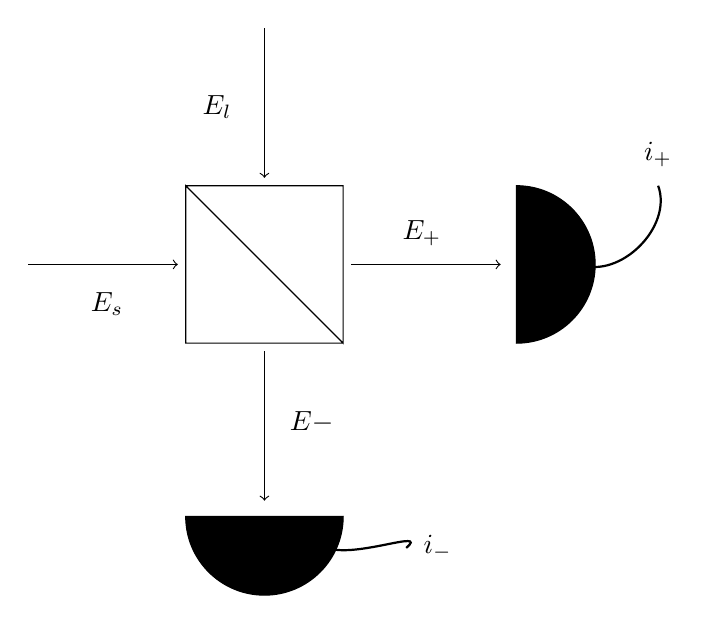
\begin{tikzpicture}
        \draw (0, 0) -- ++(2, 0) -- ++(0, -2) -- (0, 0) -- ++(0, -2) -- ++(2, 0);
        \draw[->] (-2, -1) -- ++(1.9, 0);
        \draw[->] (1, 2) -- ++(0, -1.9);
        \draw[<-] (1, -4) -- ++(0, 1.9);
        \draw[<-] (4, -1) -- ++(-1.9, 0);
        \draw[fill=black, rotate=-90, yshift=22mm] (2, 2) -- (2, 2) arc(0:180:1) --cycle;
        \draw[fill=black, rotate=-180, yshift=22mm, xshift=-20mm] (2, 2) -- (2, 2) arc(0:180:1) --cycle;
        \node at (0.4, 1) {$E_l$};
        \node at (-1, -1.5) {$E_s$};
        \node at (3, -0.6) {$E_+$};
        \node at (1.6, -3) {$E-$};
        \draw[thick] (5, -1) to[out=-20, in=-70] ++(1, 1);
        \node at (6, 0.4) {$i_+$};
        \draw[thick] (1.8, -4.6) to[out=-20, in=40] ++(1, 0);
        \node at (3.2, -4.6) {$i_-$};
    \end{tikzpicture}
\end{document}
